\documentclass[a4paper]{article}

\usepackage[utf8]{inputenc}
\usepackage{hyperref}
\usepackage{titlesec}
\usepackage[titles]{tocloft}
\usepackage{appendix}
\hypersetup{%
    pdfborder = {0 0 0}
}

\usepackage[svgnames]{xcolor} % Required to specify font color
\usepackage{listings}
\usepackage{graphicx}
\usepackage{float}

\usepackage{chngcntr}
\counterwithin{figure}{section}

\newcommand*{\plogo}{\fbox{$\mathcal{PL}$}} % Generic publisher logo

%----------------------------------------------------------------------------------------
%	TITLE PAGE
%----------------------------------------------------------------------------------------

\newcommand*{\titleAT}{\begingroup % Create the command for including the title page in the document
\newlength{\drop} % Command for generating a specific amount of whitespace
\drop=0.1\textheight % Define the command as 10% of the total text height

\rule{\textwidth}{1pt}\par % Thick horizontal line
\vspace{2pt}\vspace{-\baselineskip} % Whitespace between lines
\rule{\textwidth}{0.4pt}\par % Thin horizontal line

\vspace{\drop} % Whitespace between the top lines and title
\centering % Center all text
\textcolor{Black}{ % Red font color
{\Huge Laboratorio}\\[0.5\baselineskip] % Title line 1
{\Large di}\\[0.75\baselineskip] % Title line 2
{\Huge Calcolo Numerico}} % Title line 3

\vspace{0.25\drop} % Whitespace between the title and short horizontal line
\rule{0.3\textwidth}{0.4pt}\par % Short horizontal line under the title
\vspace{\drop} % Whitespace between the thin horizontal line and the author name

{\Large Luca De Franceschi}\par % Author name

\vfill % Whitespace between the author name and publisher text
{\large Università degli studi di Padova}\par % Publisher

\vspace*{\drop} % Whitespace under the publisher text

\rule{\textwidth}{0.4pt}\par % Thin horizontal line
\vspace{2pt}\vspace{-\baselineskip} % Whitespace between lines
\rule{\textwidth}{1pt}\par % Thick horizontal line

\endgroup}

\titleformat{\chapter}[display]
{}{\hfill\rule{.7\textwidth}{3pt}}{2pt}
{\hspace*{.3\textwidth}\huge\bfseries}[\addvspace{1pt}]
\titleformat{name=\chapter,numberless}[display]
{}{\hfill\rule{.7\textwidth}{3pt}}{2pt}
{\hspace*{.3\textwidth}\huge\bfseries}[\addvspace{1pt}]

\renewcommand*\contentsname{Indice}
\renewcommand{\figurename}{Figura}

\newcommand{\glossario}[1]{\textit{#1\ped{\ped{G}}}}

\lstset{literate=
  {á}{{\'a}}1 {é}{{\'e}}1 {í}{{\'i}}1 {ó}{{\'o}}1 {ú}{{\'u}}1
  {Á}{{\'A}}1 {É}{{\'E}}1 {Í}{{\'I}}1 {Ó}{{\'O}}1 {Ú}{{\'U}}1
  {à}{{\`a}}1 {è}{{\`e}}1 {ì}{{\`i}}1 {ò}{{\`o}}1 {ù}{{\`u}}1
  {À}{{\`A}}1 {È}{{\'E}}1 {Ì}{{\`I}}1 {Ò}{{\`O}}1 {Ù}{{\`U}}1
  {ä}{{\"a}}1 {ë}{{\"e}}1 {ï}{{\"i}}1 {ö}{{\"o}}1 {ü}{{\"u}}1
  {Ä}{{\"A}}1 {Ë}{{\"E}}1 {Ï}{{\"I}}1 {Ö}{{\"O}}1 {Ü}{{\"U}}1
  {â}{{\^a}}1 {ê}{{\^e}}1 {î}{{\^i}}1 {ô}{{\^o}}1 {û}{{\^u}}1
  {Â}{{\^A}}1 {Ê}{{\^E}}1 {Î}{{\^I}}1 {Ô}{{\^O}}1 {Û}{{\^U}}1
  {œ}{{\oe}}1 {Œ}{{\OE}}1 {æ}{{\ae}}1 {Æ}{{\AE}}1 {ß}{{\ss}}1
  {ç}{{\c c}}1 {Ç}{{\c C}}1 {ø}{{\o}}1 {å}{{\r a}}1 {Å}{{\r A}}1
  {€}{{\EUR}}1 {£}{{\pounds}}1
}

\definecolor{light-gray}{gray}{0.95}

\lstdefinestyle{customat}{
  belowcaptionskip=1\baselineskip,
  breaklines=true,
  frame=shadowbox,
  numbers=left,
  xleftmargin=\parindent,
  language=Matlab,
  showstringspaces=false,
  basicstyle=\fontfamily{georgia}\selectfont\footnotesize\color{black},
  keywordstyle=\bfseries\color{green!40!black},
  commentstyle= \color{gray},
  identifierstyle=\color{blue},
  stringstyle=\color{orange},
  tabsize=2,
  numberstyle=\tiny
}

\renewcommand{\lstlistingname}{Listato}
\renewcommand{\lstlistlistingname}{Elenco dei listati}
\renewcommand{\listfigurename}{Elenco delle figure}

\pagestyle{headings}

\AtBeginDocument{%
  \renewcommand{\thelstlisting}{%
    \ifnum\value{subsection}=0
      \thesection.\arabic{lstlisting}%
    \else
      \ifnum\value{subsubsection}=0
        \thesection.\arabic{lstlisting}%
      \else
      \thesubsubsection%
      \fi
    \fi
  }
}

%----------------------------------------------------------------------------------------
%	BLANK DOCUMENT
%----------------------------------------------------------------------------------------

\begin{document}
\raggedright
\titleAT % This command includes the title page
\thispagestyle{empty}
\newpage

\pagenumbering{arabic}

\tableofcontents
\clearpage

\lstlistoflistings
\listoffigures
\clearpage

\section{Esercitazione 1}

\subsection{Librerie di base per il calcolo seriale in Algebra Lineare Numerica (BLAS)}

Gran parte dei problemi del calcolo scientifico ed ingegneristico richiede di risolvere uno o più problemi dell'algebra lineare numerica (ALN):

\begin{itemize}

	\item Risoluzione di sistemi lineari;
	\item Risoluzione di problemi ai minimi quadrati;
	\item Ricerca di autovalori e/o autovettori;
	\item Calcolo della SVD (valori e vettori singolari);

\end{itemize}

Inoltre, la risoluzione di questi problemi è generalmente una percentuale considerevole del costo computazionale totale richiesto per la risoluzione del problema globale; questo costo si traduce spesso in ore o giorni di tempo-macchina impiegato. Dunque, implementare in modo efficiente gli algoritmi che risolvono i problemi dell'algebra lineare numerica è estremamente importante dal punto di vista applicativo ed è anche per questo che trattiamo questo caso più approfonditamente.
Un secondo motivo è dovuto al fatto che esistono in rete delle librerie che rappresentano lo stato dell'arte per questi problemi e sono molto ben costruite anche dal punto di vista della implementazione e distribuzione del software numerico: BLAS, LAPACKe ATLAS (disponibili al sito www.netlib.org/blas , /lapack e /atlas).

Gli algoritmi di algebra lineare numerica hanno in comune un insieme relativamente piccolo e stabile di operazioni di base, che svolge la quasi totalità dei calcoli necessari negli algoritmi di ALN. Questo fatto giustifica lo sforzo di creazione di una libreria che implementi queste funzione di base. La libreria BLAS è organizzata in tre livelli:
operazioni che lavorano su vettori e producono uno scalare  (es. il prodotto interno, o scalare, tra due vettori colonna: v' * w), operazioni tra vettori e matrici o che comunque producono una matrice (es. il prodotto esterno tra due vettori colonna: v * w'), operazioni tra matrici (es. il prodotto di due matrici).

Un vantaggio rilevante di aver creato la BLAS è che questa può essere ottimizzata per ogni singola macchina ed in questo modo gli algoritmi di ALN possono diventare ``portabili'' anche dal punto di vista delle prestazioni di calcolo e non solo da quello della sintassi, semplicemente chiamando le routines della BLAS ove possibile.

Ora, ha senso chiedersi se le operazioni di livello 1, 2 o 3 raggiungono le stesse prestazioni di calcolo. Lo vediamo implementando lo stesso identico algoritmo, il prodotto di due matrici C = A * B, in tre modi diversi, corrispondenti all'utilizzo esclusivo di operazioni di livello 1, di livello 2 e di livello 3.

\begin{figure}[ht!]
\centering
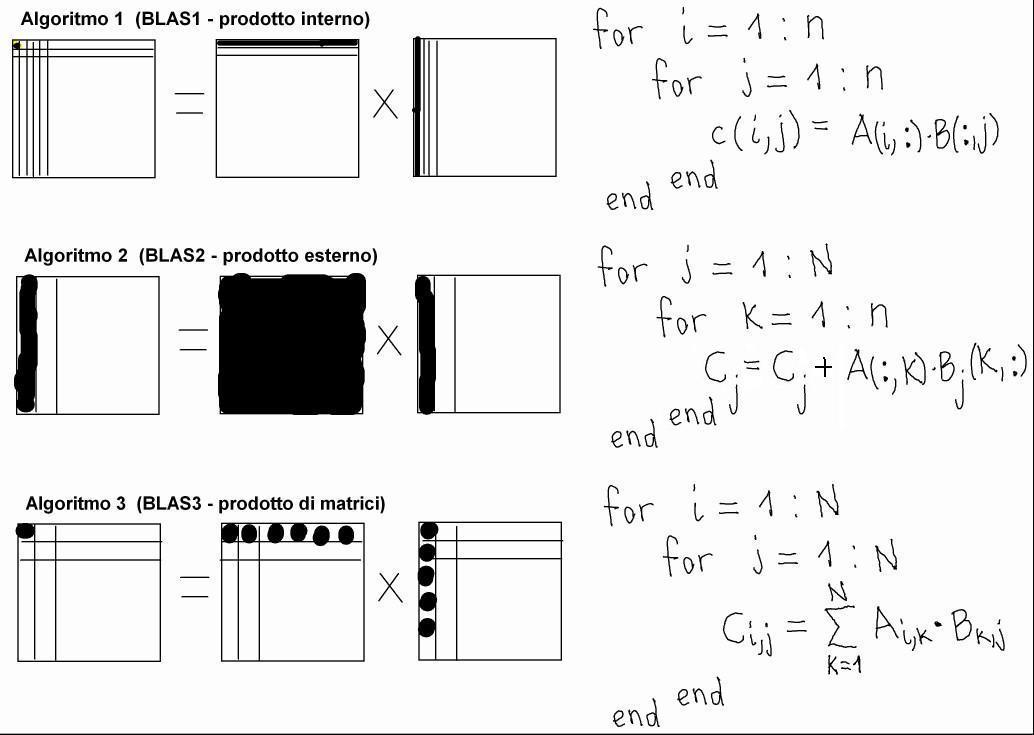
\includegraphics[width=130mm]{images/implementazioni_prodotto_di_matrici.jpg}
\caption{Algoritmi BLAS}
\label{overflow}
\end{figure}
\newpage
\section{Esercitazione 2}

\subsection{Ambienti software dedicati al calcolo scientifico}

È ben noto che per creare programmi al ``calcolatore'' sia necessario disporre di un ``ambiente di programmazione''. Tale ambiente, in parte inserito nel sistema operativo ed in parte costituito da software aggiuntivo, fornisce strumenti indispensabili alla creazione e verifica dei programmi, come: un editor, un compilatore, un linker, un debugger, ...     

Un ambiente software dedicato al calcolo scientifico aggiunge a questi strumenti degli altri strumenti dedicati allo sviluppo di applicazioni che utilizzano principalmente le capacità di calcolo del calcolatore.
Da non confondere l'ambiente software dedicato al calcolo scientifico con la libreria di calcolo scientifico, che fornisce ``solamente'' un insieme di metodi numerici, richiamabili da un programma. 

Per applicazioni del calcolo scientifico vengono tipicamente utilizzate assieme più d'una libreria. Ambienti molto diffusi di questo tipo sono: \textbf{Matlab} (il capostipite, 1983 ca., commerciale), \textbf{Octave} (open-source), \textbf{Scilab} (open-source). Recentemente, si sta affermando l'utilizzo di \textbf{Python}, grazie alla sua shell interattiva ed alle estensioni numeriche disponibili.

\subsubsection{Il workspace}

L’ambiente di calcolo, che si presenta con una linea di comando, mantiene disponibili in memoria tutte le variabili che sono state inizializzate dal momento dell'ingresso nell’ambiente, sia tramite singoli comandi che tramite istruzioni contenute nei programmi eseguiti, entrambi impartiti dalla linea di comando dell'ambiente. Questa è una sostanziale differenza rispetto alla programmazione in C o in FORTRAN, dove le variabili vengono allocate all’inizio dell’esecuzione del programma e poi de-allocate (cioè cancellate) al termine dell’esecuzione stessa. Una conseguenza immediata di questo fatto è che, ad esempio, in un ambiente come il Matlab non è necessario salvare esplicitamente su file i valori delle variabili che si vogliono osservare (es. graficare) dopo l’esecuzione del programma.


\subsubsection{La grafica}

Non è sufficiente produrre dei (buoni) risultati numerici, bensì è anche necessario poterli osservare a valutare in modo adeguato. Solitamente questa operazione richiede la produzione di qualche tipo di grafico, per cui l’esistenza di capacità grafiche è un elemento fondamentale di un ambiente software dedicato al calcolo scientifico. Matlab possiede capacità grafiche evolute ed Octave si appoggia a Gnuplot (applicativo anch’esso open-source).

\subsubsection{L’esecuzione dei programmi}

Per mandare in esecuzione un programma scritto per Matlab o per Octave (e quindi un file di testo con il suffisso ``.m'' contenente istruzioni che rispettano la sintassi del linguaggio di Matlab, ovvero un ``m-file'') è sufficiente scrivere il nome del m-file sulla riga di comando e premere il tasto invio. Se il programma non è nella directory corrente, è necessario prima mettersi nella directory che lo contiene.
Il calcolo dei tempi di esecuzione è semplice, e quindi è possibile misurare la velocità di esecuzione dell’algoritmo numerico: conoscendo il numero di operazioni floating-point (flops) richieste per il calcolo della soluzione, si può calcolare la velocità:

\begin{center} 

$MFLOPS = numeroDiLops / tempoTrascorso$.

\end{center}

Notare che il tempo di esecuzione di un algoritmo numerico è oggi il principale parametro per misurarne l'efficienza. Infatti, mentre fino a qualche anno fa le operazioni in virgola mobile venivano fatte via software/firmware, e dunque una moltiplicazione costava più di un'addizione, ora sono implementate via hardware, e dunque richiedono sostanzialmente lo stesso numero di cicli di clock del processore. Pertanto, mentre fino a qualche tempo fa il parametro più usato era il numero di operazioni floating-point richieste, ora lo è il tempo di esecuzione dove, attenzione, pesano anche gli aspetti non numerici dell'algoritmo (esistenza di istruzioni di scelta, movimento dei dati da e verso la memoria, ...).

Per quanto riguarda l'ambiente di calcolo, è necessario tenere presente che Matlab (ed Octave) eseguono il programma utente in maniera interpretata, e cioè viene letta, compilata ed eseguita un’istruzione alla volta. Questo incide moltissimo sulla velocità di esecuzione di un algoritmo. In particolar modo è bene evitare di creare troppi cicli innestati.

\subsubsection{Il linguaggio di programmazione ``domain specific''}

L’ambiente Matlab (Octave) mette a disposizione un linguaggio di programmazione che da un lato contiene tutti i costrutti tipici della programmazione strutturata (if-then-else, ciclo for, ciclo while, ecc...) e dall’altro permette di manipolare in modo molto semplice e sintetico le strutture dati fondamentali per il calcolo matriciale, e cioè vettori e matrici, in modo analogo a quanto viene fatto dal linguaggio tradizionale più evoluto per il calcolo, il Fortran90 e successive varianti, ed a quanto può essere fatto a partire dai linguaggi orientati agli oggetti, come il C++ , Java, ...

Il linguaggio di Matlab (Octave) offre il vantaggio, rispetto ai linguaggi di programmazione tradizionali, di semplificare molto l’uso del linguaggio per la costruzione di un programma, lasciando quindi l’attenzione del programmatore libera il più possibile dagli aspetti puramente informatici e concentrata sugli aspetti algoritmici e numerici. Anche per questo è molto diffuso, sia come strumento di studio che come strumento di lavoro, in particolare per la prototipazione dei codici di calcolo. Per un utilizzo in ``produzione'', i compilatori dei linguaggi tradizionali sono però preferibili perchè permettono di ottimizzare maggiormente il codice eseguito dalla macchina e dunque, generalmente, l’algoritmo implementato viene eseguito più velocemente (che, nella realtà delle applicazioni, è molto rilevante).


\subsection{Rappresentazione dei numeri al calcolatore}

I calcolatori oggi in commercio rispettano in genere il medesimo standard per la rappresentazione dei numeri in virgola mobile ( floating-point ): lo standard \textbf{IEEE 754}.

Nello standard IEEE la precisione singola occupa una parola da 32 bit, mentre la precisione doppia occupa due parole consecutive da 32 bit. Un numero non-nullo normalizzato ``X'' ha la seguente rappresentazione binaria:

\begin{center}
	\textbf{S E F}
	\\
	$X  =  (-1)^S  *  2^(E-bias)  *  (1.F)$
	\end{center}

dove bias = 127 (single) o 1023 (double).

Lo standard richiede che il risultato delle operazioni di addizione, sottrazione, moltiplicazione e divisione sia arrotondato esattamente, cioè il risultato deve essere calcolato esattamente e poi arrotondato al numero in virgola mobile più vicino.

Problemi in tal senso provengono dalla sottrazione. Per questo motivo, nei microprocessori moderni la sottrazione viene effettuata utilizzando la tecnica bit di guardia:  l'operando più piccolo viene troncato a p+1 cifre binarie, mentre il risultato della sottrazione viene troncato a p cifre (binarie). In realtà, il calcolo con un solo bit di guardia non sempre produce lo stesso risultato che si avrebbe calcolando il risultato esatto e poi arrotondando a p cifre binarie. Introducendo un secondo bit di guardia ed un terzo bit sticky, si ottiene il pieno rispetto dello standard con un extra-costo computazionale relativamente piccolo.

\subsection{Propagazione degli errori di arrotondamento}

Ogni calcolatore ha a disposizione un numero finito M di cifre per rappresentare un numero reale. Se il numero da rappresentare possiede più di M cifre significative, il calcolatore lo arrotonda alle M cifre più significative. A causa di questo fatto, le operazioni aritmetiche di base sono in generale soggette ad un errore nel risultato, ed è dunque necessario conoscere l’entità di questo errore e, considerando un intero algoritmo,  l’effetto potenziale della propagazione di questo tipo di errore sul risultato finale.
In generale, la somma, la divisione e la moltiplicazione producono un errore relativo piccolo, mentre la sottrazione può anche produrre un errore relativo grande, rispetto al risultato (ciò avviene quando i due operandi sono molto vicini tra di loro e si ha dunque una notevole perdita di cifre significative nel risultato).

Il fatto che l’errore relativo nel risultato sia piccolo non è comunque una garanzia di accuratezza  in generale: la somma tra due operandi troppo distanti in magnitudo può addirittura far scomparire dal risultato il più piccolo dei due ed avere comunque un errore relativo piccolo. Per questo motivo, ad esempio,  quando si deve eseguire una sommatoria, è buona regola eseguirla mettendo gli operandi in ordine crescente, in modo che la somma parziale ed il prossimo numero da sommare siano il più vicini possibile in magnitudo.

Vediamo di seguito alcuni esempi relativi a questi fenomeni:

\subsubsection{Calcolo delle radici di un’equazione di secondo grado}

Vediamo ora un esempio concreto di calcolo in cui introdurre una sottrazione potenzialmente pericolosa conduca effettivamente a problemi di instabilità della soluzione, e come rimediare.

Data: $a*x^2 + b*x +c$ , calcolare le sue radici.

La formula classica, $x = (- b \pm sqrt(b^2 – 4*a*c))/(2*a)$ , è potenzialmente instabile a causa della sottrazione tra b/2 e sqrt(...) . Provare ad implementarla e verificarne la perdita di accuratezza per opportune scelte dei coefficienti a, b, e c.

Ripetere poi lo stesso tipo di indagine su una formula alternativa, stabile, che si ottiene calcolando prima la radice positiva ( in cui non si effettua la sottrazione) e poi calcolando l’altra sapendo che vale :  

\begin{center}
	$c = a * x_1 * x_2$.
\end{center}

\lstinputlisting[style=customat, caption=Equazioni di secondo grado]{../Esercitazione2/equazioniSecondoGrado.m}

\subsubsection{Approssimazione del pigrego}

È un altro esempio di sottrazione pericolosa, questa volta in un metodo numerico iterativo per l’approssimazione di pi-greco. Provare ad implementare i seguenti tre metodi iterativi ed a graficarne l’errore relativo, in scala logaritmica, per le prime 100 iterate (un valore molto accurato di pi-greco in Matlab/Octave è contenuto nella variabile di sistema “pi”). Per n = 2,3,4,.... calcolare le tre approssimazioni di pi-greco, y(n), w(n) e z(n):

\begin{enumerate}
	\item $s(2)=1+1/4;$ \\ $s(n+1)=s(n)+1/((n+1)^2);$ \\ $y(n+1)= sqrt(6*s(n+1));$
	\item $w(2)=2;$ \\ $w(n+1)=2^(n-1/2)*sqrt(1-sqrt(1-4^(1-n)*w(n)^2));$
	\item $z(2)=2;$ \\ $z(n+1)=(sqrt(2)*z(n))/(sqrt(1+sqrt(1-4^(1-n)*z(n)^2)));$
	\linebreak[4]
	\linebreak[4]
\end{enumerate}


\lstinputlisting[style=customat, caption=Approssimazione del pigreco]{../Esercitazione2/SuccessionePigreco.m}

\subsubsection{Successioni calcolabili praticamente}

Si consideri la seguente successione:

\begin{center}
	$y(0)=1/e*(e-1);$
	\\
	$y(n+1)=1-(n+1)*y(n);$
\end{center}

Essa converge (in aritmetica con infinite cifre) a zero per n->inf. Implementarla e verificare cosa accade nel calcolatore, cercando di giustificare i risultati. Inoltre, sapendo che y(n) è circa =0 per n sufficientemente grande, provare ad implementarla all'indietro e vedere cosa risulta per y(0). Perchè?

\lstinputlisting[style=customat, caption=Successioni calcolabili]{../Esercitazione2/SuccessioniAvantiIndietro.m}
\newpage
\section{Esercitazione 3}

Spesso ci sono situazioni in cui guardando certe proprietà del problema numerico da risolvere, si possono trovare degli accorgimenti che risultano avere un impatto non trascurabile sul costo computazionale dell'algoritmo di calcolo. Vediamo di seguito un paio di esempi di questo tipo:

\subsection{Prodotto matrice-vettore}

Supponiamo che sia necessario compiere il prodotto matrice-vettore $A*b$,  in cui la matrice ``A'', di dimensione n x n, è un campionamento della funzione:

\begin{center}  

$f(x,y) = cos(x)*cos(y)$

\end{center}

in una griglia cartesiana di punti nell'intervallo $[0, pi] x [0, pi]$, e ``b'' è un vettore colonna di lunghezza n. Scelti:

\begin{itemize}
\item Un vettore riga di coordinate ``x'' avente n elementi scelti nell'intervallo $[0, pi]$,  e calcolato il vettore ``vx'' tale che  $vx(i) = cos(x(i))$;
\item Un vettore riga di coordinate ``y'' avente n elementi scelti nell'intervallo $[0, pi]$,  e calcolato il vettore ``vy'' tale che  $vy(i) = cos(y(i))$;
\end{itemize}

allora la matrice ``A'' può essere espressa nella forma:

\begin{center}
$A  =  vx' * vy$
\end{center}

dove l'apice significa ``trasposto''.  In generale, essendo A una matrice densa, il prodotto $A*b$ per un generico vettore ``b'' ha un costo dell'ordine di  $O(n^2)$. 

Se, però, utilizziamo l'espressione con cui viene costruita ``A'' ed invertiamo la precedenza nei calcoli:

\begin{center}
$vx' * (vy * b)$
\end{center}

otteniamo una complessità dell'ordine di $O(n)$.
\newline

\textbf{Esercizio}: costruire un programma Matlab/Octave che esegua il prodotto matrice-vettore $A*b$ nelle due modalità qui prospettate e verifichi automaticamente che il risultato del prodotto nei due casi è il medesimo. Inoltre, verificare sperimentalmente, per alcuni valori di n, se l'andamento dei tempi di esecuzione segue l'andamento della complessità qui prospettato e costuire un grafico $(n, tempi)$.

\lstinputlisting[style=customat, caption=Prodotto matrice-vettore]{../Esercitazione3/esercizio1.m}

\begin{figure}[H]
\centering
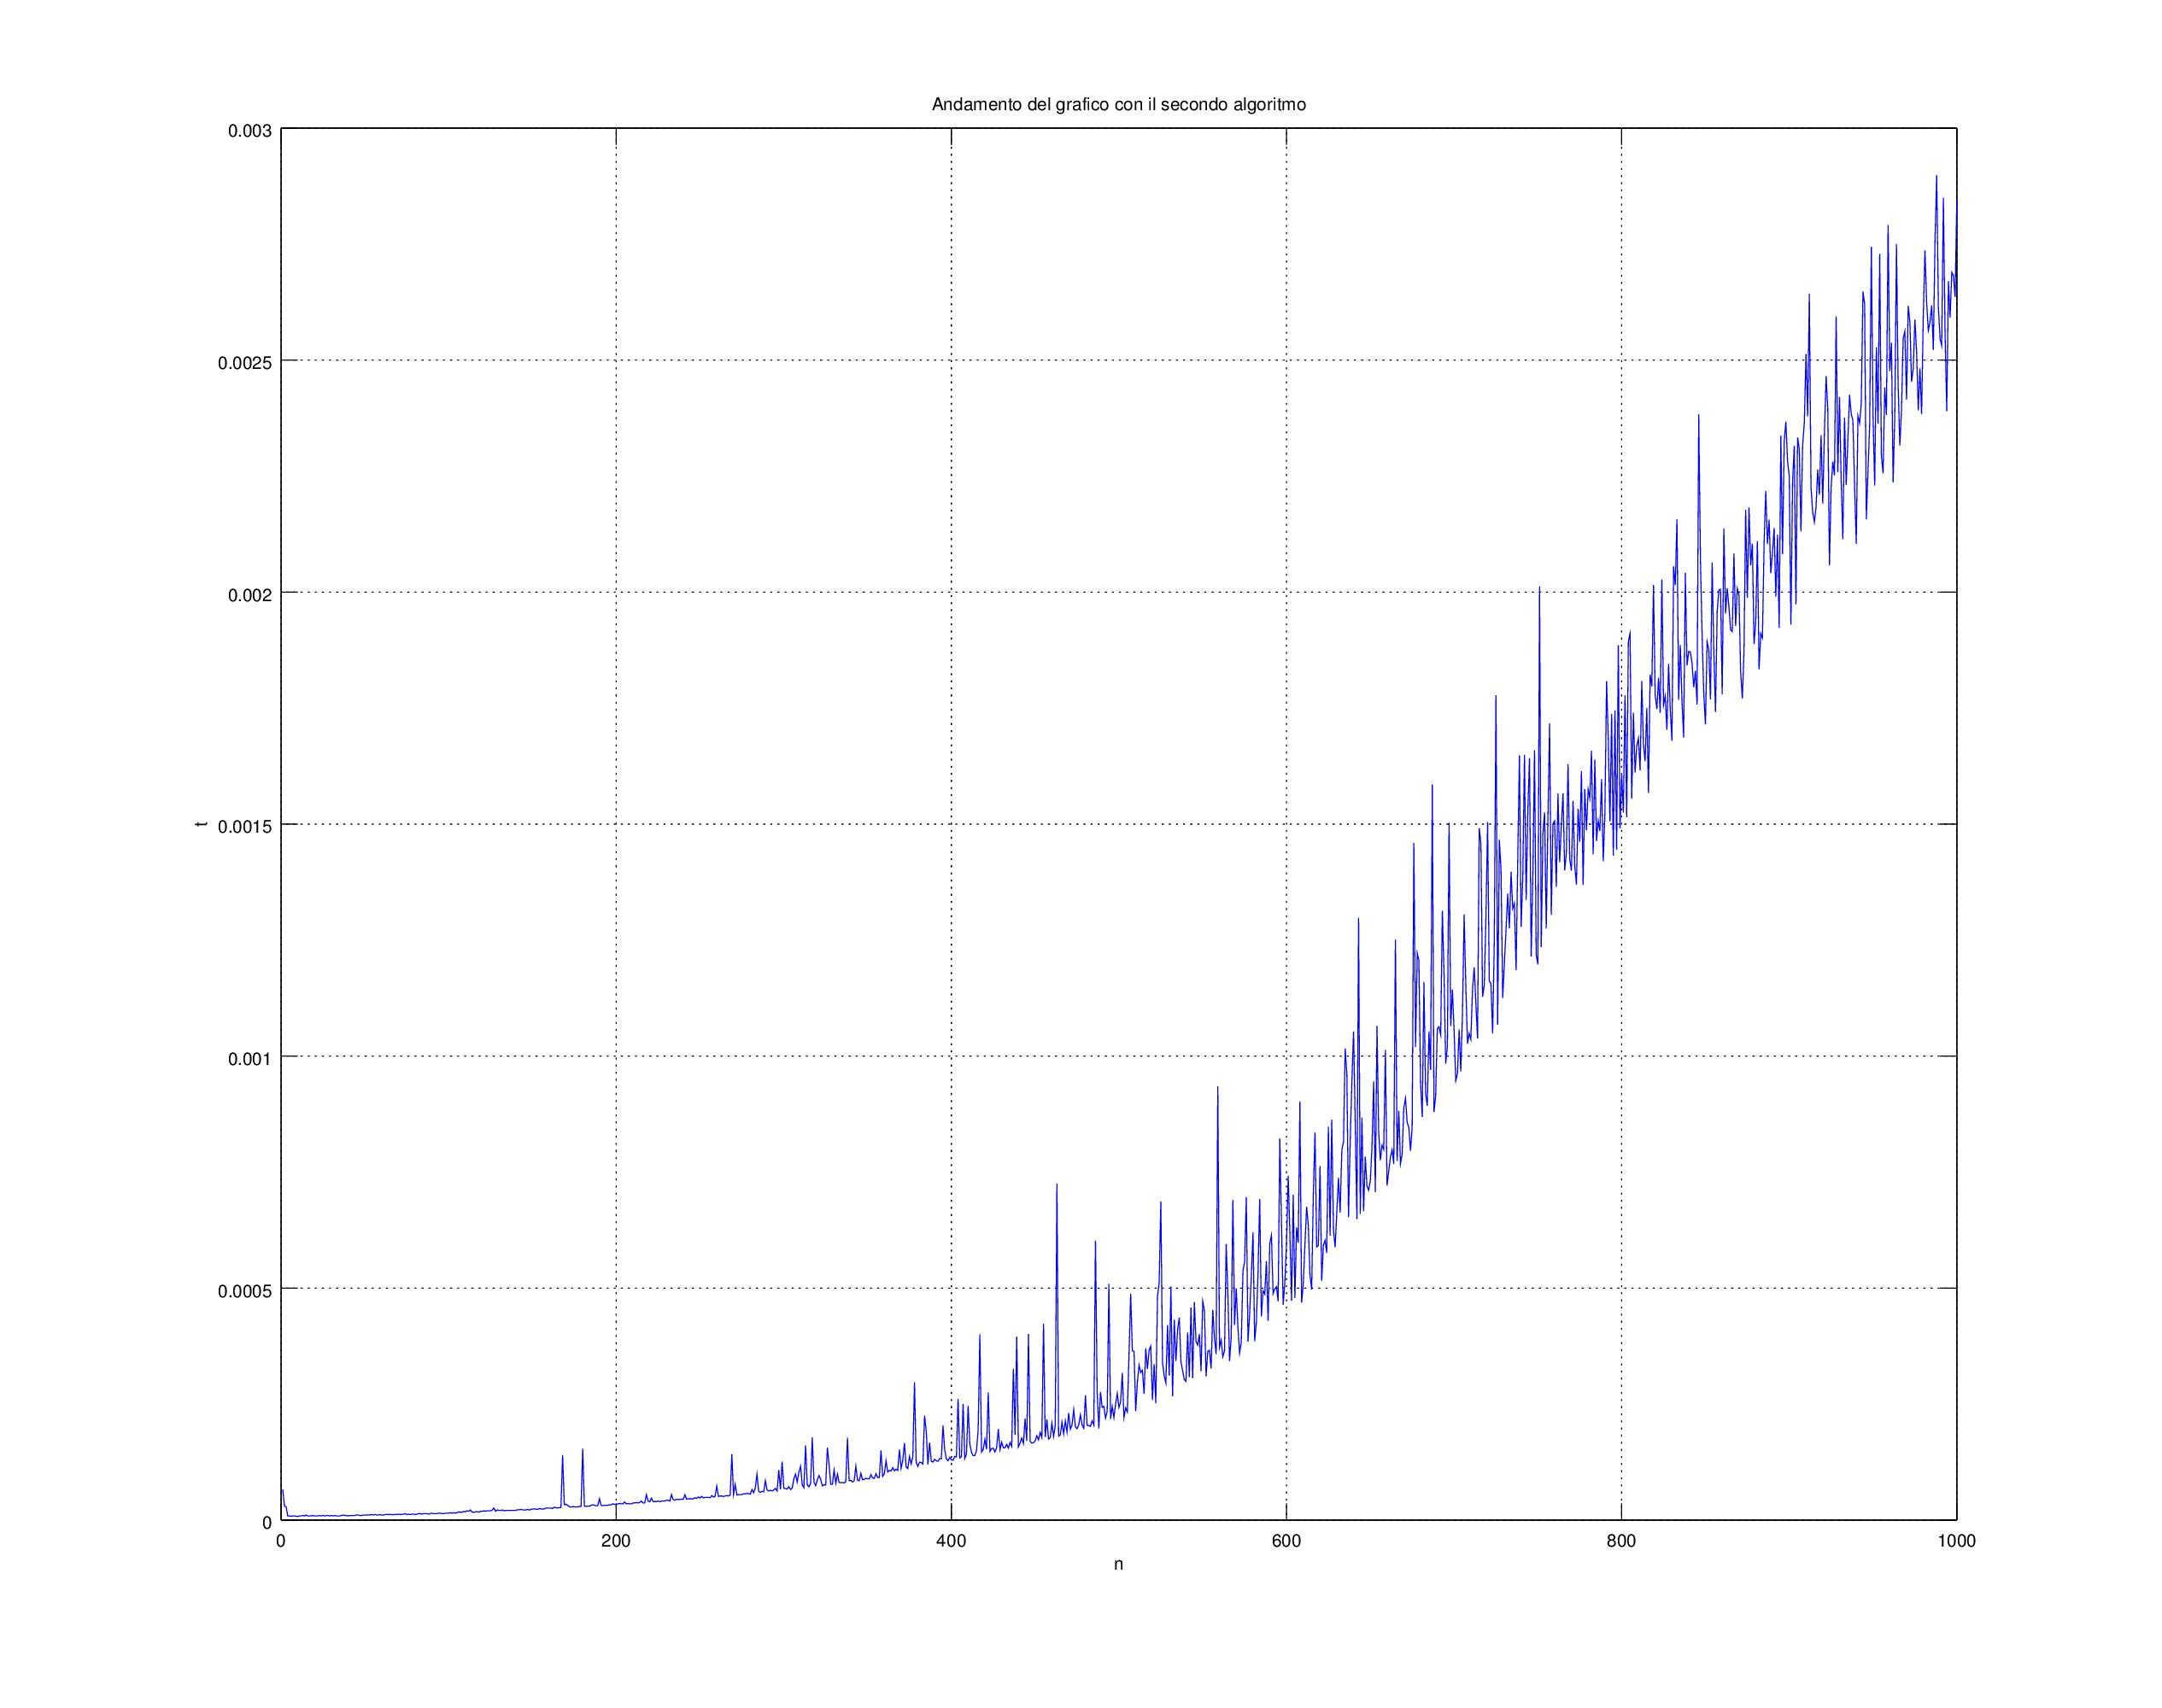
\includegraphics[width=100mm]{../Esercitazione3/images/esercizio1a.jpg}
\caption{Andamento dei tempi nel caso 1}
\label{overflow}
\end{figure}

\begin{figure}[H]
\centering
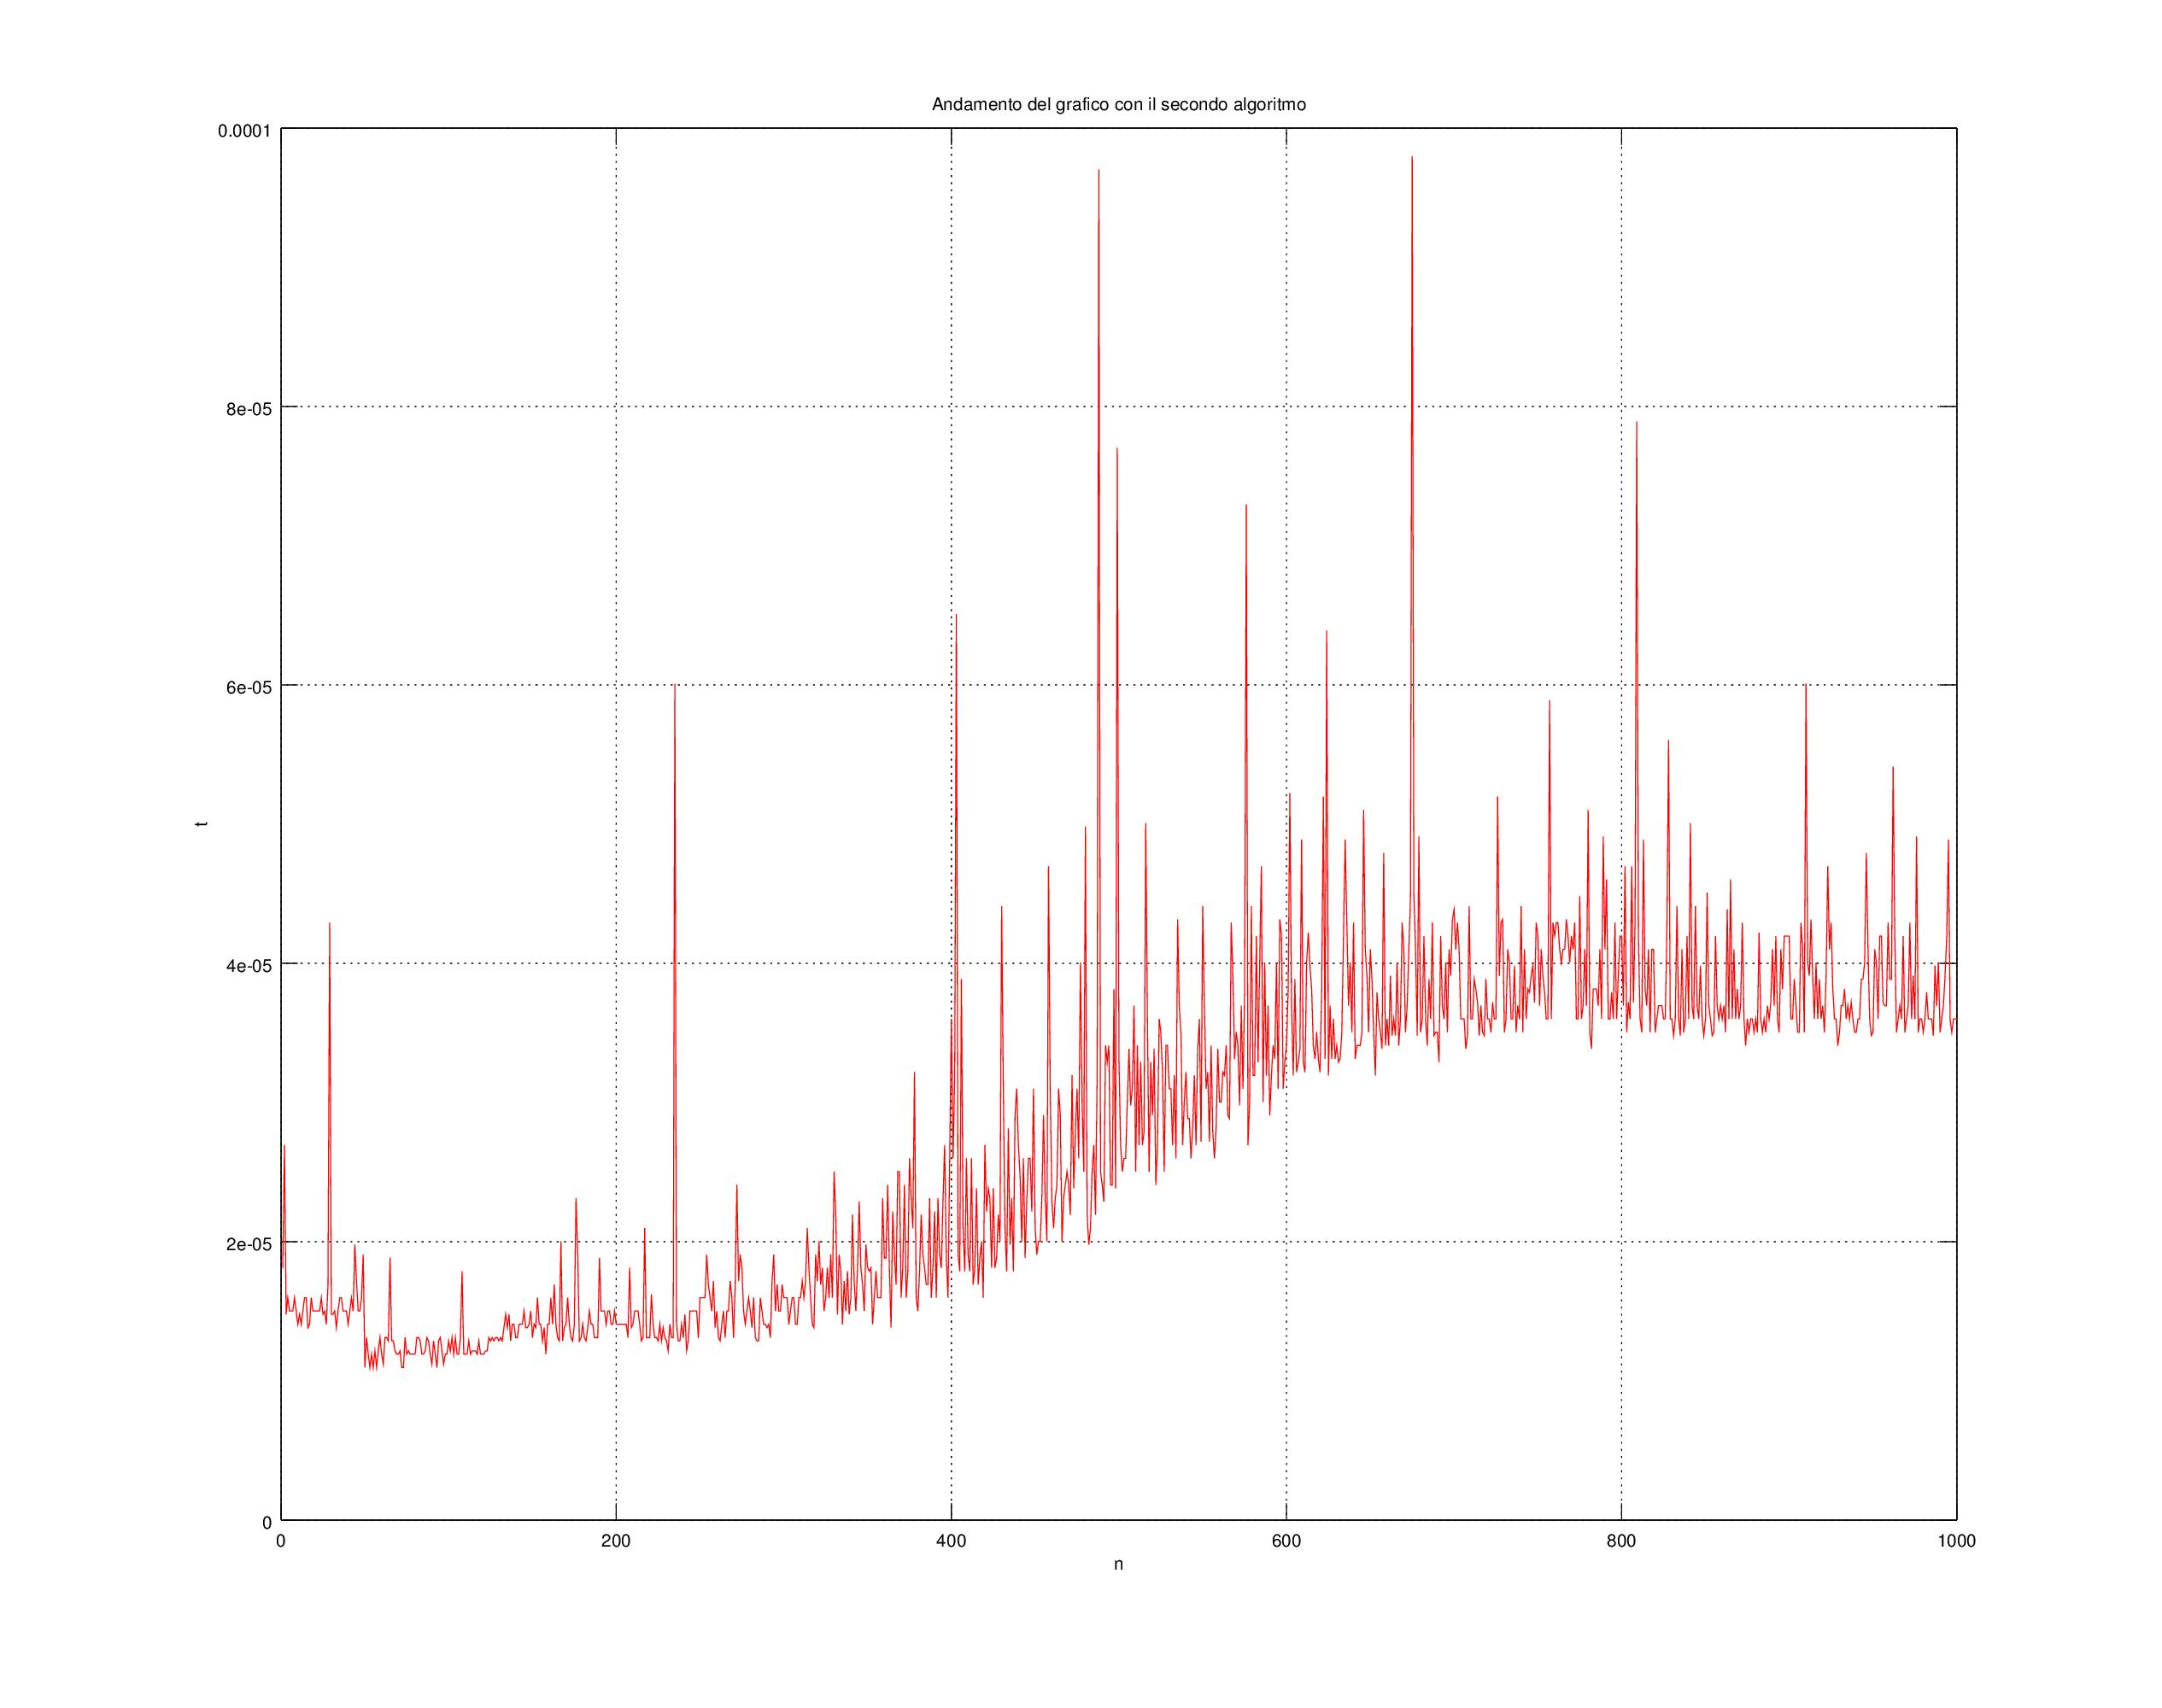
\includegraphics[width=100mm]{../Esercitazione3/images/esercizio1b.jpg}
\caption{Andamento dei tempi nel caso 2}
\label{overflow}
\end{figure}

\begin{figure}[H]
\centering
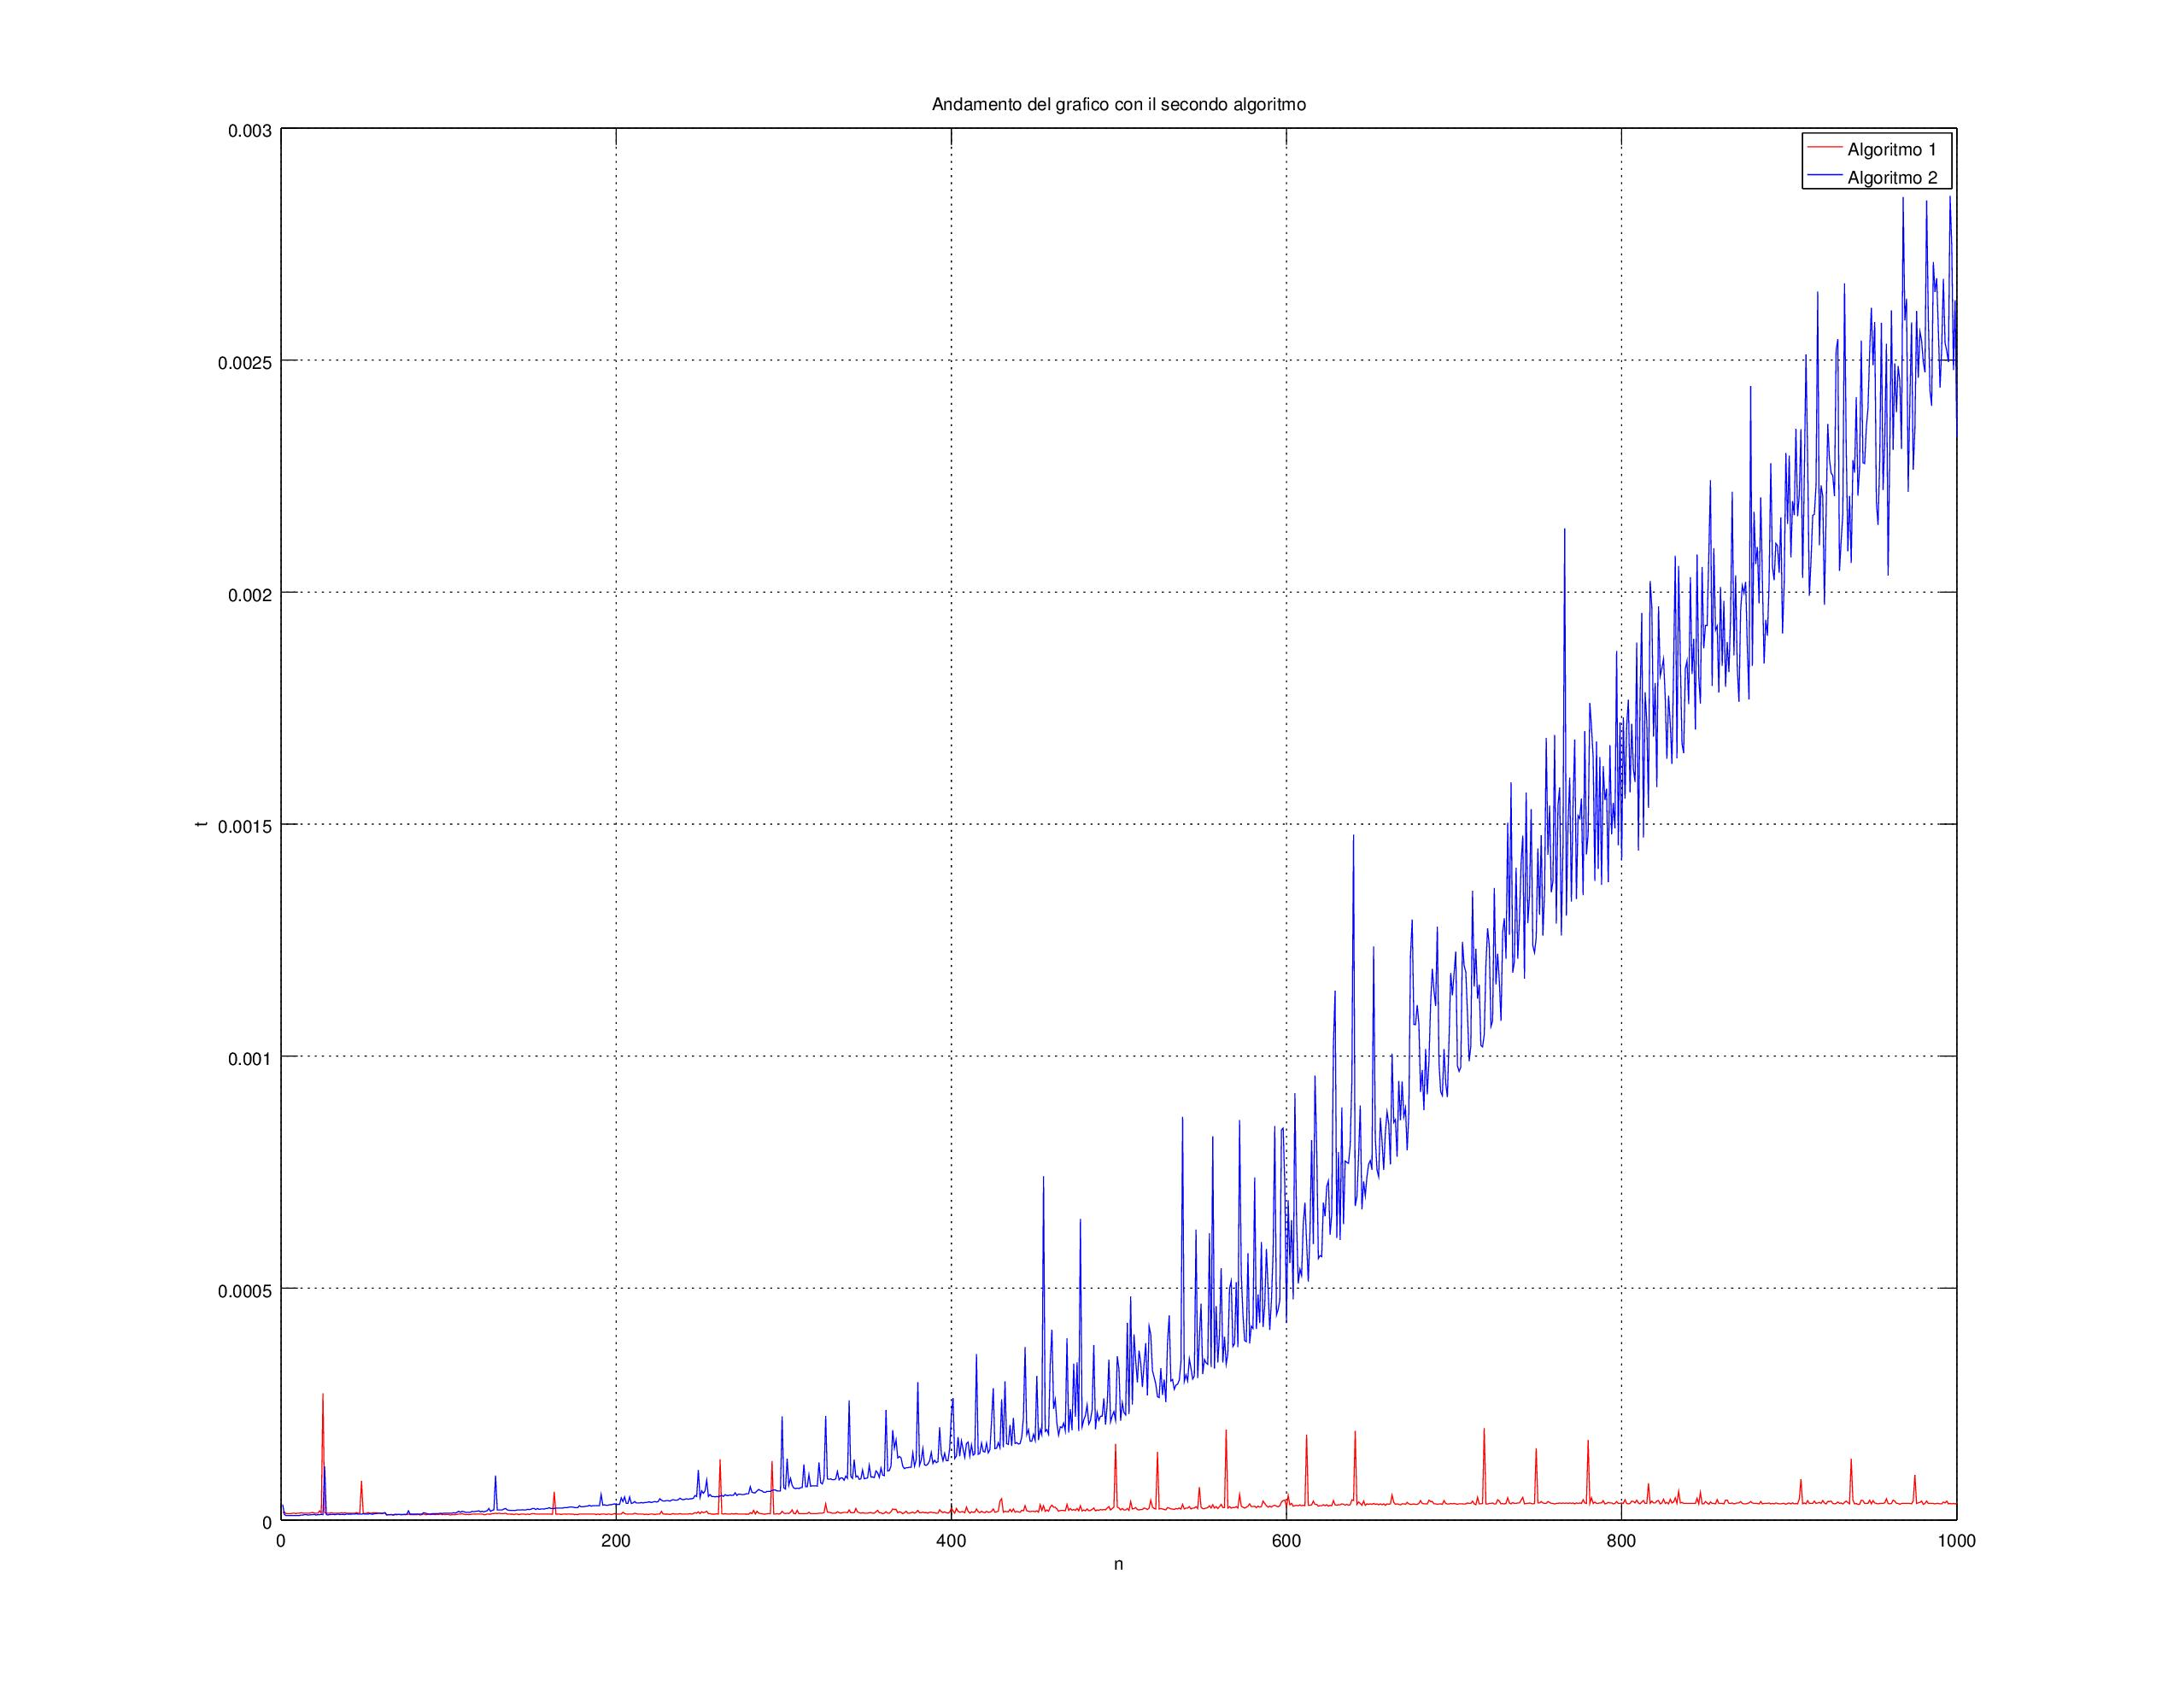
\includegraphics[width=100mm]{../Esercitazione3/images/esercizio1c.jpg}
\caption{Confronto degli andamenti dei due algoritmi}
\label{overflow}
\end{figure}

\subsection{Potenze di matrici}

Per calcolare la potenza q-esima, $q \geq 1$, di una matrice ``A'', si può pensare di moltiplicare ``A'' q-1 volte per se stessa.

In modo più efficiente, possiamo esprimere ``q'' in base-2 (cioè in formato binario), calcolarci i termini $A^{(2^{i})}$,  $i =  1,...,\log{2(q)}-1 = \log{q}/\log{2} -1$ mediante la:

\begin{center}

$A^{(2^i)}  =  A^{(2^{(i-1)})}  *  A^{(2^{(i-1)})}$

\end{center}

e sfruttare il fatto che:

\begin{center}
$A^{(c1 + c2 + c3)}  =  A^{c1}  *  A^{c2}  *  A^{c3}$
\end{center}

\textbf{Esercizio}:  costruire un programma Matlab/Octave che, data una generica matrice ``A'' ed assegnato un valore di ``q'', esegua il calcolo di $A^q$  nelle due modalità qui esposte e verifichi automaticamente che il risultato nei due casi è il medesimo. Inoltre, valutare dal programma qual'è la complessità dei due algoritmi e verificare sperimentalmente, con una matrice ``A'' a scelta e valori di $q = 4,5,...15$ ,  se l'andamento dei tempi di esecuzione segue l'andamento della complessità atteso. Costuire un grafico $(n, tempi)$.

\lstinputlisting[style=customat, caption=Potenze di matrici]{../Esercitazione3/esercizio2.m}

\end{document}